\documentclass[../main.tex]{subfiles}
\graphicspath{{\subfix{../Images/}}}
\begin{document}
\section{Functions}

\subsection{Set Notation}
\begin{tabular}{|c|c|c|}
    \hline
    \textbf{Symbol} & \textbf{Meaning} & \textbf{Example} \\
    \hline
    \(\mathbb{N}\) & Natural Numbers & \(\{1,2,3, \cdots\}\) \\
    \hline
    \(\mathbb{Z}^{+}_{0}\) & Non -ve Integers & \(\{0,1,2, \cdots\}\) \\
    \hline
    \(\mathbb{Z}\) & Integers & \(\{\cdots ,-1,0,1, \cdots\}\) \\
    \hline
    \(\mathbb{Q}\) & Rationals & \(\{\frac{p}{q} : \, p,q \in \mathbb{Z}\}\) \\
    \hline
    \(\mathbb{R}\) & Real Numbers & \(\{\cdots, -\pi, \frac{1}{2}, \sqrt{2}, 2 \cdots\}\) \\
    \hline
    \(\mathbb{C}\) & Complex Numbers & \(\{a+bi : \, a,b \in \mathbb{R}\}\) \\
    \hline
\end{tabular} \\
\boxedeq{\mathbb{N} \subset \mathbb{Z}^{+}_{0} \subset \mathbb{Z} \subset \mathbb{Q} \subset \mathbb{R} \subset \mathbb{C}}

\subsubsection{Interval Notation}
\begin{tabular}{|c|c|}
    \hline
    \textbf{Notation} & \textbf{Definition} \\
    \hline
    \([a,b]\) & \(\{x\in\mathbb{R} : a \leq x \leq b\}\) \\
    \hline
    \((a,b)\) & \(\{x\in\mathbb{R} : a < x < b\}\) \\
    \hline
    \((a,b]\) & \(\{x\in\mathbb{R} : a < x \leq b\}\) \\
    \hline
    \((-\infty,b]\) & \(\{x\in\mathbb{R} : x \leq b\}\) \\
    \hline
    \([a,b) \cup (c,\infty)\) & \(\{x\in\mathbb{R} : a \leq x < b \text{ or } x > c\}\) \\
    \hline
    \([a,c) \cap [b,\infty)\) & \(\{x\in\mathbb{R} : b \leq x < c\}\) \\
    \hline
    \(\mathbb{R}\backslash\{0\}\) & \(\{x\in\mathbb{R} : x \neq 0\}\) \\
    \hline
\end{tabular} \\\\
\textbf{Notes} \\
Interval and Set Notations are not exact replacements \\* of each other even though they are similar

\subsection{Definitions}
\subsubsection{Notations}
\begin{tabular}{|c|c|}
    \hline
    \textbf{Representation} & \textbf{Meaning} \\
    \hline
    \(f\) & function \\
    \hline
    \(f:A \to B\) & Set Mapping \\
    \hline
    \(f:x \mapsto x^2\) & Rule of function \\
    \hline
    \(f(x)\) & Rule of function \\
    \hline
    \(D_{f}\) & Domain of \(f\) \\
    \hline
    \(R_{f}\) & Range of \(f\) \\
    \hline
\end{tabular}
\newpage \noindent

\subsubsection{Relations}
The Associatation between 2 Sets is a Relation \\
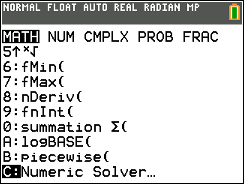
\includegraphics[scale=0.7]{2 Functions/Capture 1.png}

\subsubsection{Definition of a Function}
A \textbf{Function} is a relation from Set \(X\) to \(Y\) where every input \(x \in X\) is mapped to a \textbf{unique output} \(y \in Y\) \\\\
With this definition, we can see from 3.2.2 that only (a) \& (b) are functions.
(c) is not a function as input \((x=-1)\) is mapped to \(y=-1\) \& \(y=1\), (d) in
not a function as input \((x=5)\) does not have a related output in \(Y\) \\\\
%Function Notation%
Function Example:
\begin{align*}
    \displaystyle f:x \mapsto x, \, & x \in (-2,2) \\
        \text{Rule}\phantom{spa} & \phantom{s }\text{Domain}
\end{align*}

\subsubsection{Finding Range with GC}
Key the function into the GC, while taking note of the starting and ending points of the domain.
If the function has turning points, it has to be taken into account as it coul affect the Range. \\\\
Example: \\
\(\displaystyle f:x \mapsto e^{x^{2}+2x+1}\), \(x \in [-2,0.5)\) \\
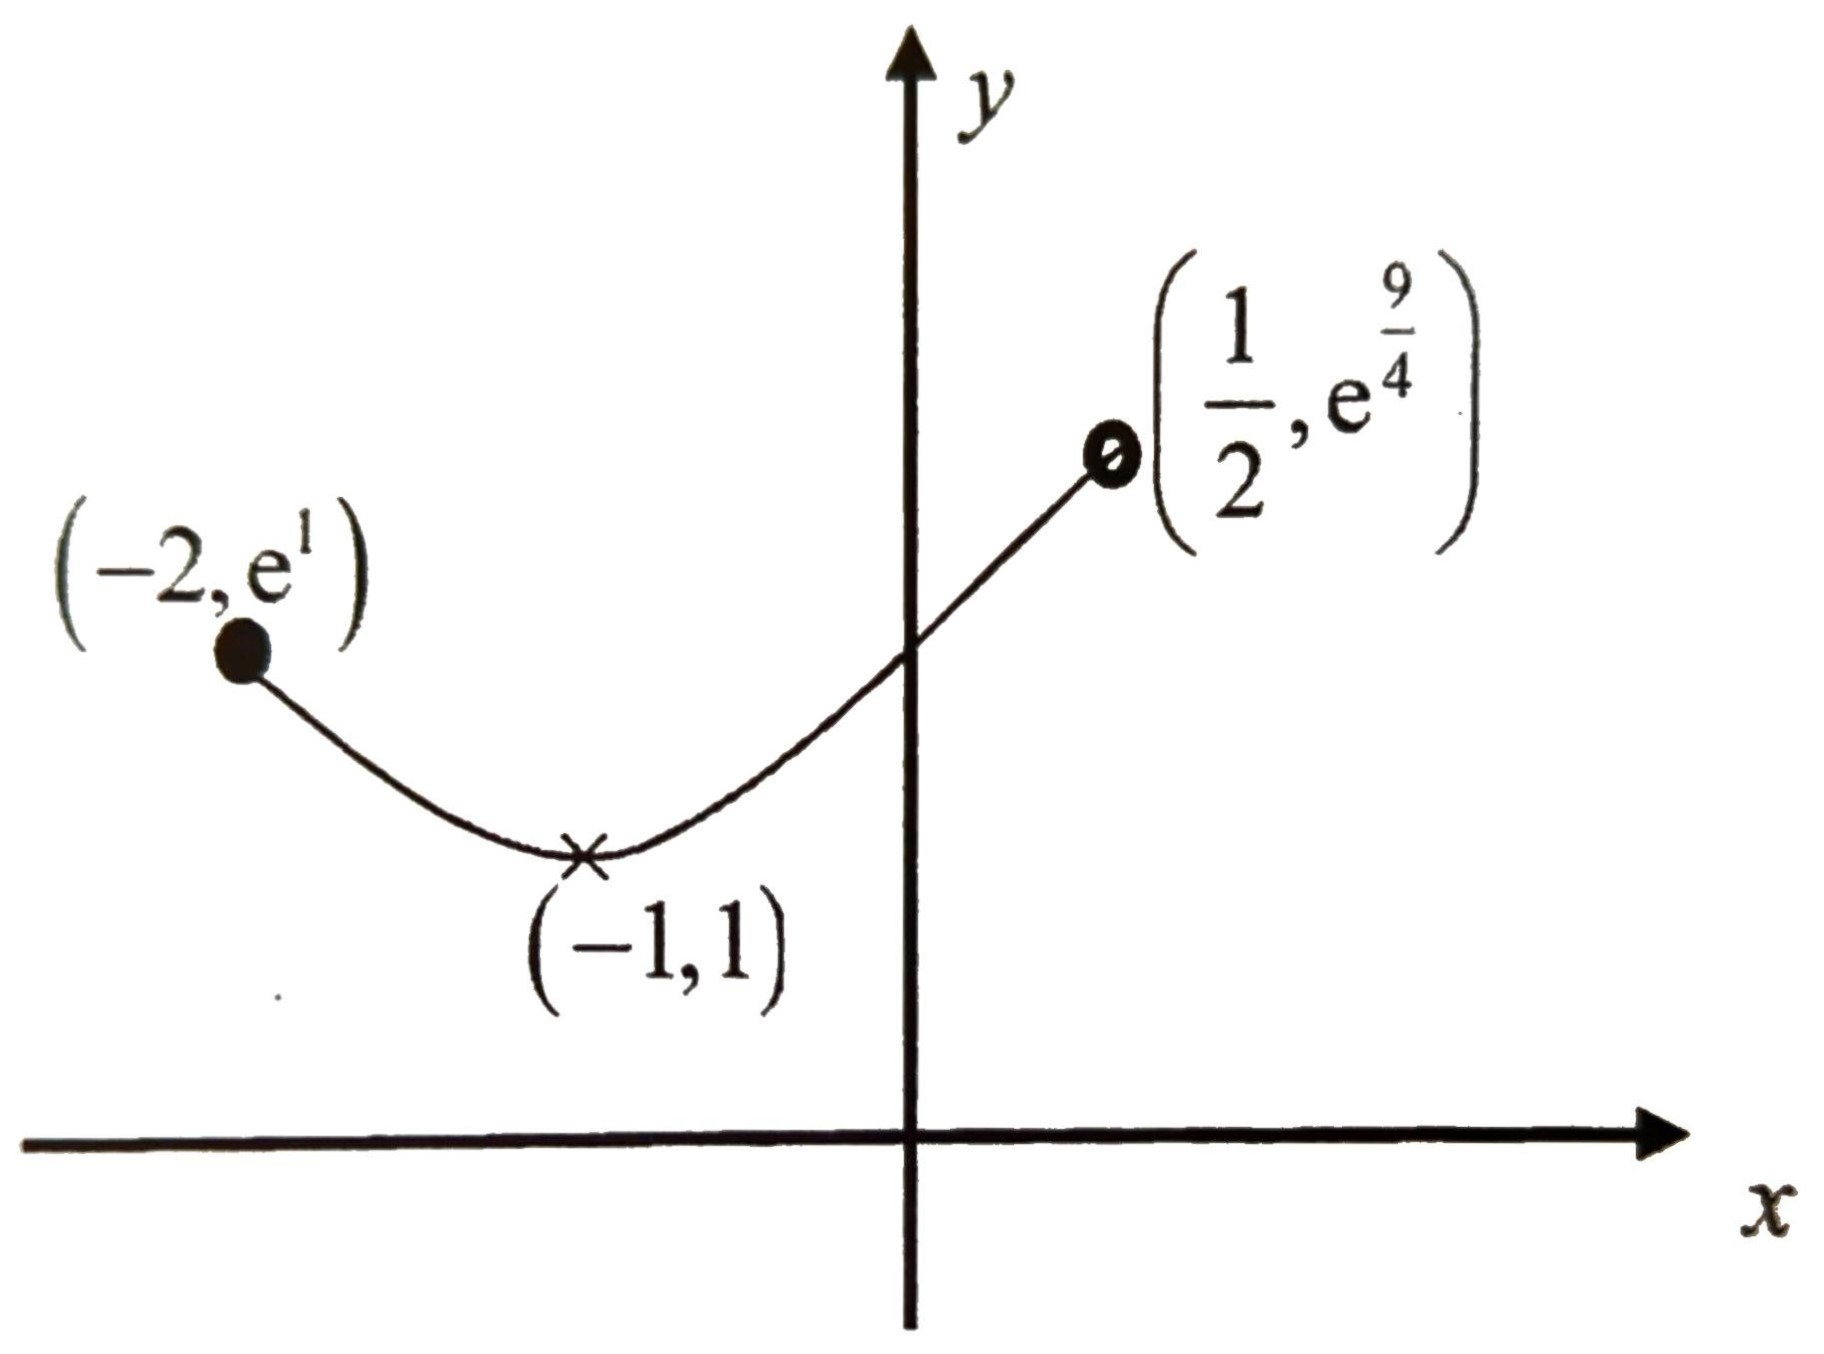
\includegraphics[scale=0.1]{2 Functions/Capture 2.jpg} \\
\(\therefore R_{f} = \left[1,e^{\textstyle \frac{9}{4}}\right)\)

\subsection{Injective Functions}
\subsubsection{Definition of Injection}
Injectivity means that every input has a \textbf{unique} output \\*
formally, \(f: X \mapsto Y\) is injective iff
\boxedeq{f(a)=f(b) \implies a=b \text{ OR } a \neq b \implies f(a) \neq f(b)}
where \(a,b, \in \mathbb{D}_{f}\)

\subsubsection{Disproving Injectivity}
We only need to show that a single value violates the \\*
definition, which can be done by the horizontal line test \\

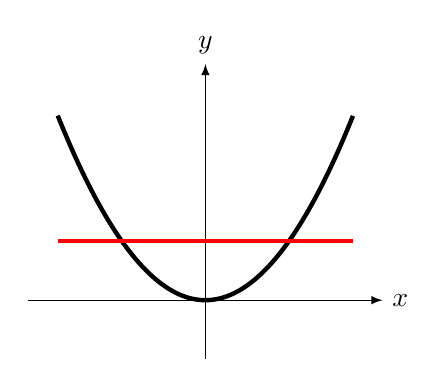
\begin{tikzpicture}[scale=0.75]
    % Draw axes
    \draw[-latex] (-3,0) -- (3,0) node[right] {\(x\)};
    \draw[-latex] (0,-1) -- (0,4) node[above] {\(y\)};

    % Draw y=x^2
    \draw[samples=100,domain=-2.5:2.5,smooth,variable=\x,black,ultra thick] plot ({\x},{0.5*\x*\x});

    % Draw y=1
    \draw[samples=100,domain=-2.5:2.5,smooth,variable=\x,red,ultra thick] plot ({\x},{1});
\end{tikzpicture} \\*
In this case, as the horizontal line intercepts the function\\*
at more than 1 point, the function isn't injective

\subsubsection{Proving Injevtivity}
To prove injectivity, we would have to use the definition \\
Example, \(\displaystyle f(x) = \frac{1}{x-2}\), \(x \in \mathbb{R}\)
\begin{align*}
    \displaystyle f(a) &= f(b) \\
    \displaystyle \implies \frac{1}{a-2} &= \frac{1}{b-2} \\
    \displaystyle \implies a-2 &= b-2 \\
    \displaystyle \implies a &= b
\end{align*}
Thus, the function \(f\) is injective

\subsection{*Surjective Functions}
\subsubsection{Definition of Surjection}
Surjectivity means that the range of the function is an
equal set to the codomain. \\*
Formally, \(f: X \mapsto Y\) is surjective iff \(R_{f} \equiv Y\)

\subsection{*Bijective Functions}
\subsubsection{Definition of Bijection}
A Bijective function is one that satisfies both injectivity
and surjectivity. A function has to be bijective for the inverse
to exist, however, in the context of A-Levels, injectivity suffices

\subsection{Inverse Functions}
An inverse function, when applied to it's respective non-inverse, gives
the input of the original function, or basically undoing the function

\subsubsection{Invese Function Notation}
The inverse of a function \(f\) can be written as \(f^{-1}\)

\subsubsection{Conditions for an inverse to exist}
A function has to be bijective (or injective only in the
context of A-Levels) for the inverse to exist

\subsubsection{Properties of Inverse Functions}
\begin{enumerate}
    \item \(f^{-1}(x)\) is a reflection of \(f(x)\) about the line \(y=x\)
    \item \(\displaystyle D_{f^{-1}}=R_{f}\) and \(\displaystyle R_{f^{-1}}=D_{f}\)
    \item \(\displaystyle \left(f^{-1}\right)^{-1}=f\)
\end{enumerate}

\subsubsection{Self-Inversing functions}
A self inversing function \(f\) is one where \(ff=x\) \(\forall x \in D_{f}\) \\
Example of Self-Inversing Function : \(\displaystyle f(x) = \frac{-mx+a}{bx+m}\), where \(a,b,m\in\mathbb{R}\) \\
However, there is a value of \(a\) to omit, which is where \(-mx+a = k(bx+m)\), \(k\in\mathbb{R}\slash\{0\}\) : or \(\displaystyle a=-\frac{m^2}{b}\)

\subsection{Composite Functions}
\subsubsection{Composite Function Notation}
The composition of two functions \(f\) \& \(g\) can be written
as \(f \circ g\) or \(fg\) where \(fg(x)=f[g(x)]\) \\

\subsubsection{Conditions for a composition to exist}
For composition \(f \circ g\) to exist, \(R_{g}=D_{f}\)

\subsubsection{Properties of Composite Functions}
\begin{enumerate}
    \item Composition is not Commutative \(\displaystyle f \circ g \neq g \circ f\)
\end{enumerate}

\subsubsection{Finding Domain \& Range of a Composition}

\subsection{Extensions}

\subsubsection{Properties of Functions}

\subsubsection{Inverse Trigonometic Functions}

\subsubsection{Monotonic Functions}

\subsubsection{*Floor and Ceiling Functions}

\subsubsection{*Continuity \& Discontinuity}


\end{document}